\section{GPU 计算能力}

本章将探讨 GPU 领域中的一个关键术语——计算能力（Compute Capability，简称 CC 编号）。它是 NVIDIA 对 GPU 
架构采用的一种设计分类，表明 GPU 的通用特性和处理能力。为了更深入地理解这一点，我们先从这个问题开始：

计算能力是如何编号或赋予版本号的？

\subsection{计算能力编号}

计算能力以版本号的形式表示，例如 3.0、5.1 或 7.5。小数点前的第一个数字通常表示重大的架构变更，而小数点后的第二个数
字代表较小的改进或扩展。每个版本对应特定一代的 GPU 及其所支持的功能。以 Volta 架构为例，其计算能力被标记为 7。Volta 
因引入了张量核心（Tensor Core）而备受瞩目，大幅提升了特定类型计算的性能，尤其是在人工智能和深度学习领域。这一数字标识
反映了该架构在发布时所引入的一系列前沿特性、能力与改进。

转向 Ampere 架构，其计算能力版本为 8.0。这一提升表明与 Volta 相比，该架构在硬件和软件方面均实现了显著增强：包括更高效
、更强大的张量核心，更大的内存带宽，更高的能效等。这些增强不仅提升了性能，还提高了 GPU 在更广泛应用场景中的效率与通用
性。CC 编号这一概念适用于所有其他架构。

\begin{figure}
    \centering
    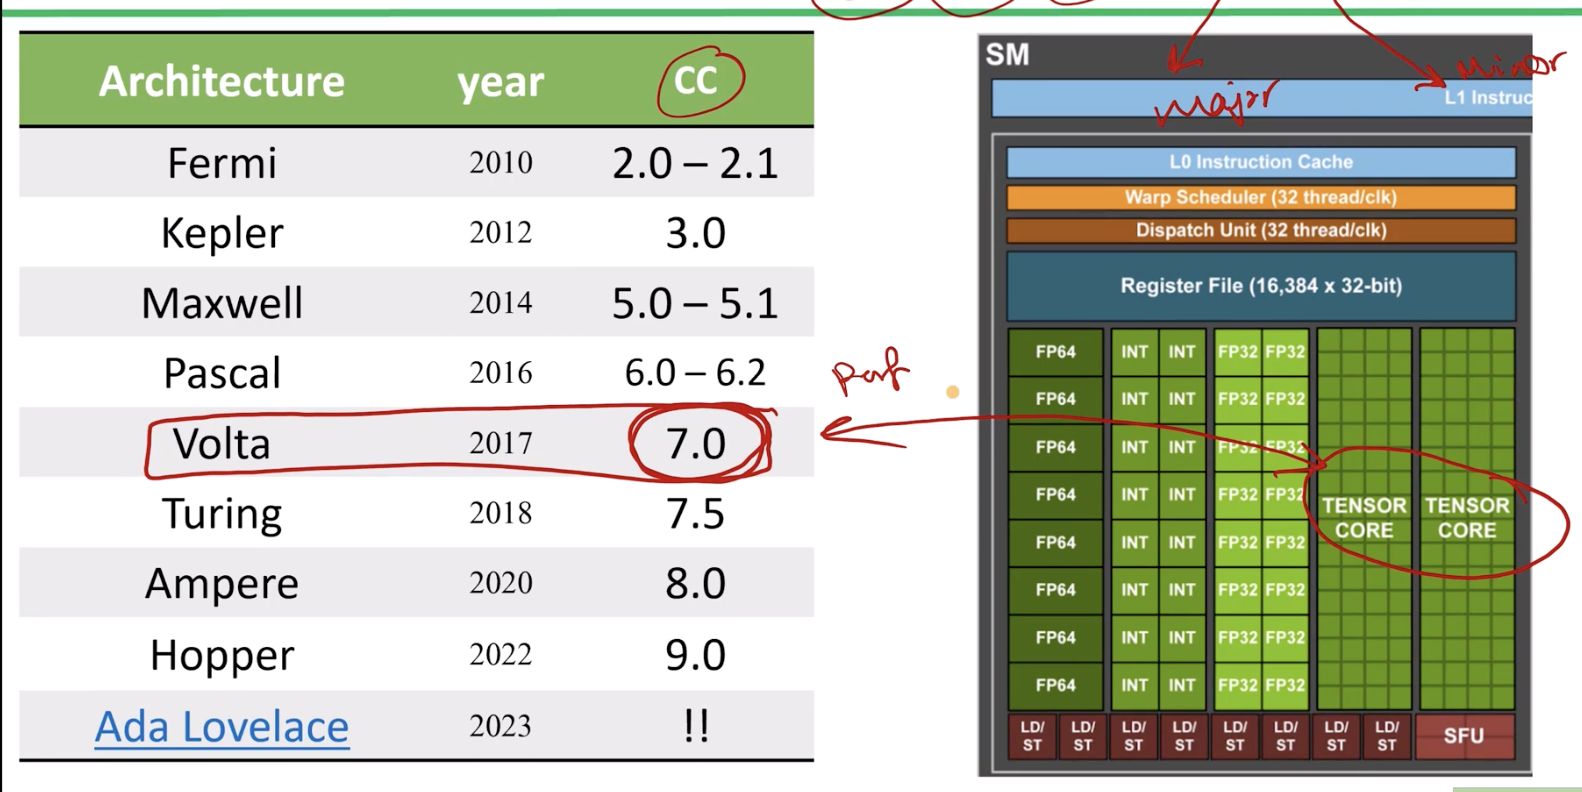
\includegraphics[width=0.75\linewidth]{resources/cuda-039.png}
    \caption{CC版本}
    \label{fig:placeholder}
\end{figure}

\subsection{功能支持}

接下来是本章的第二点——功能支持。不同版本的计算能力支持不同的功能，包括 GPU 能执行的数学运算类型、可处理的并行程度、
内存访问能力等等。例如，当你访问 CUDA 编程文档时会发现许多关于 GPU 编程的章节，其中一节专门介绍计算能力。

\begin{figure}
    \centering
    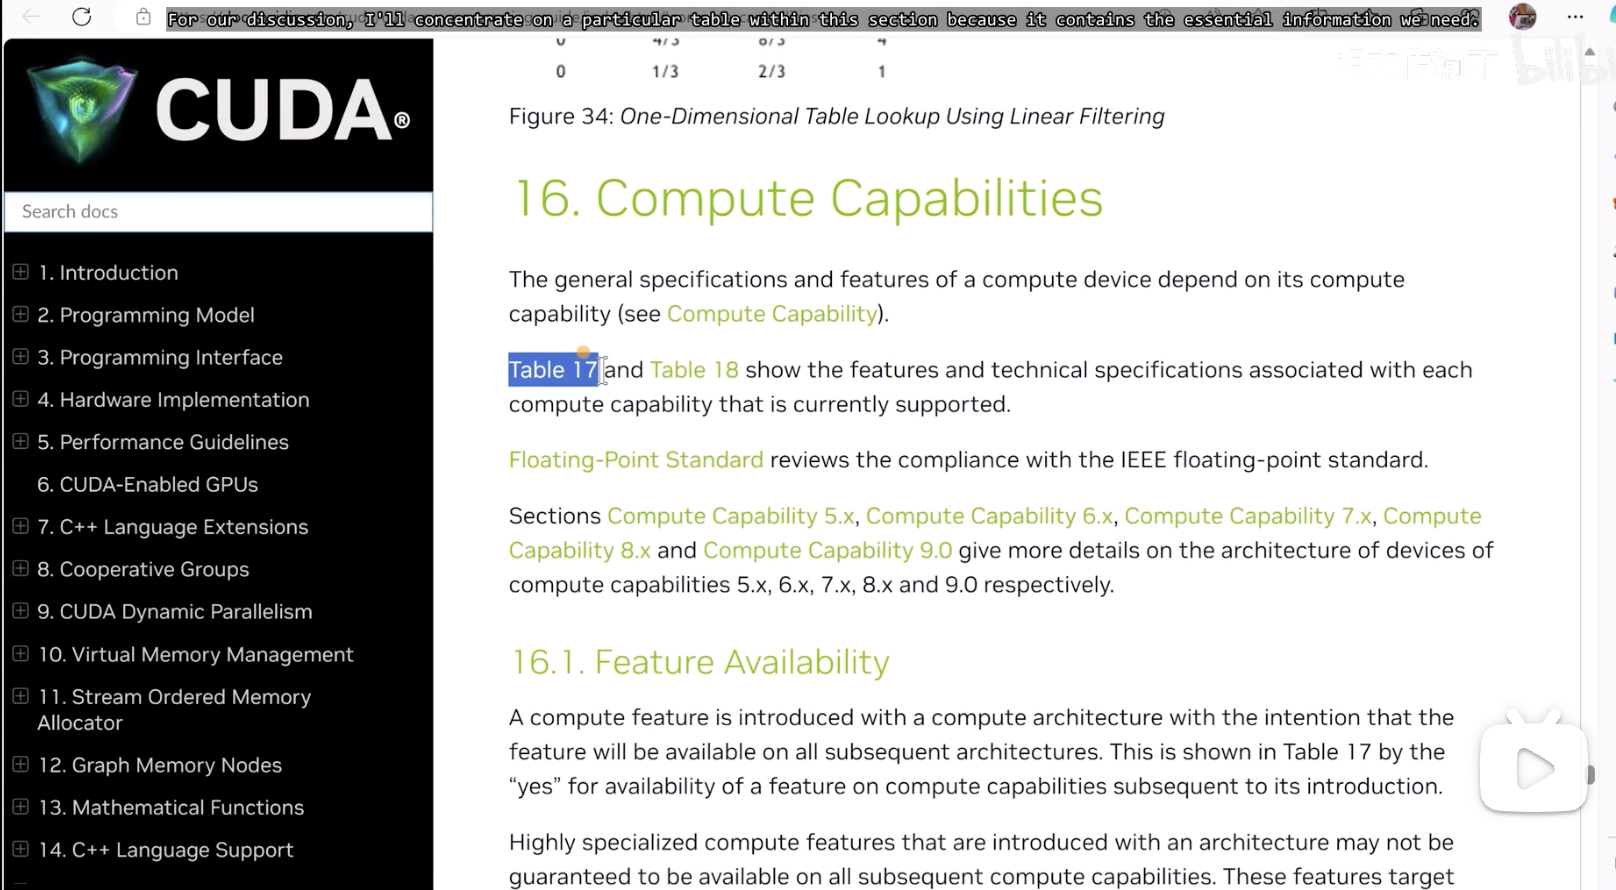
\includegraphics[width=0.75\linewidth]{resources/cuda-040.png}
    \caption{cuda 编程手册}
    \label{fig:placeholder}
\end{figure}


我将聚焦于该节中的一个特定表格，它包含了关键信息。在表 17 中，你可以看到一个结构化的布局——不同计算能力版本列于各列，
对应的功能列于各行。该表格充当对比图表，使开发者能够快速查看特定计算能力的 GPU 支持哪些功能。以计算能力 5.0 为例，从
上到下逐行扫描会发现其中混杂着可用与不可用的功能：具备该计算能力的 GPU 不支持半精度运算，如表所示，在代表计算能力低于
7 的各列中，该项标记为 No。张量核心是另一类重要单元，仅从计算能力 7 及以上版本才开始提供（对应列中标记为 Yes）。表 18 
也体现了相同的概念，留待读者自行查阅。


\subsection{软件兼容性}

更高的计算能力版本能够兼容更新的 CUDA 工具包，而新版本工具包又支持更先进的计算功能和更优的性能优化。换言之，GPU 的计算
能力决定了它可运行的 CUDA 工具包的版本。为了说明这一概念，以 PTX 兼容性为例——为简化理解，可将 PTX 视作一种 GPU 汇编
语言。部分 PTX 指令只能在特定计算能力版本的设备上执行，因为它们依赖于仅存在于特定计算能力 GPU 上的硬件单元或功能。

\begin{figure}
    \centering
    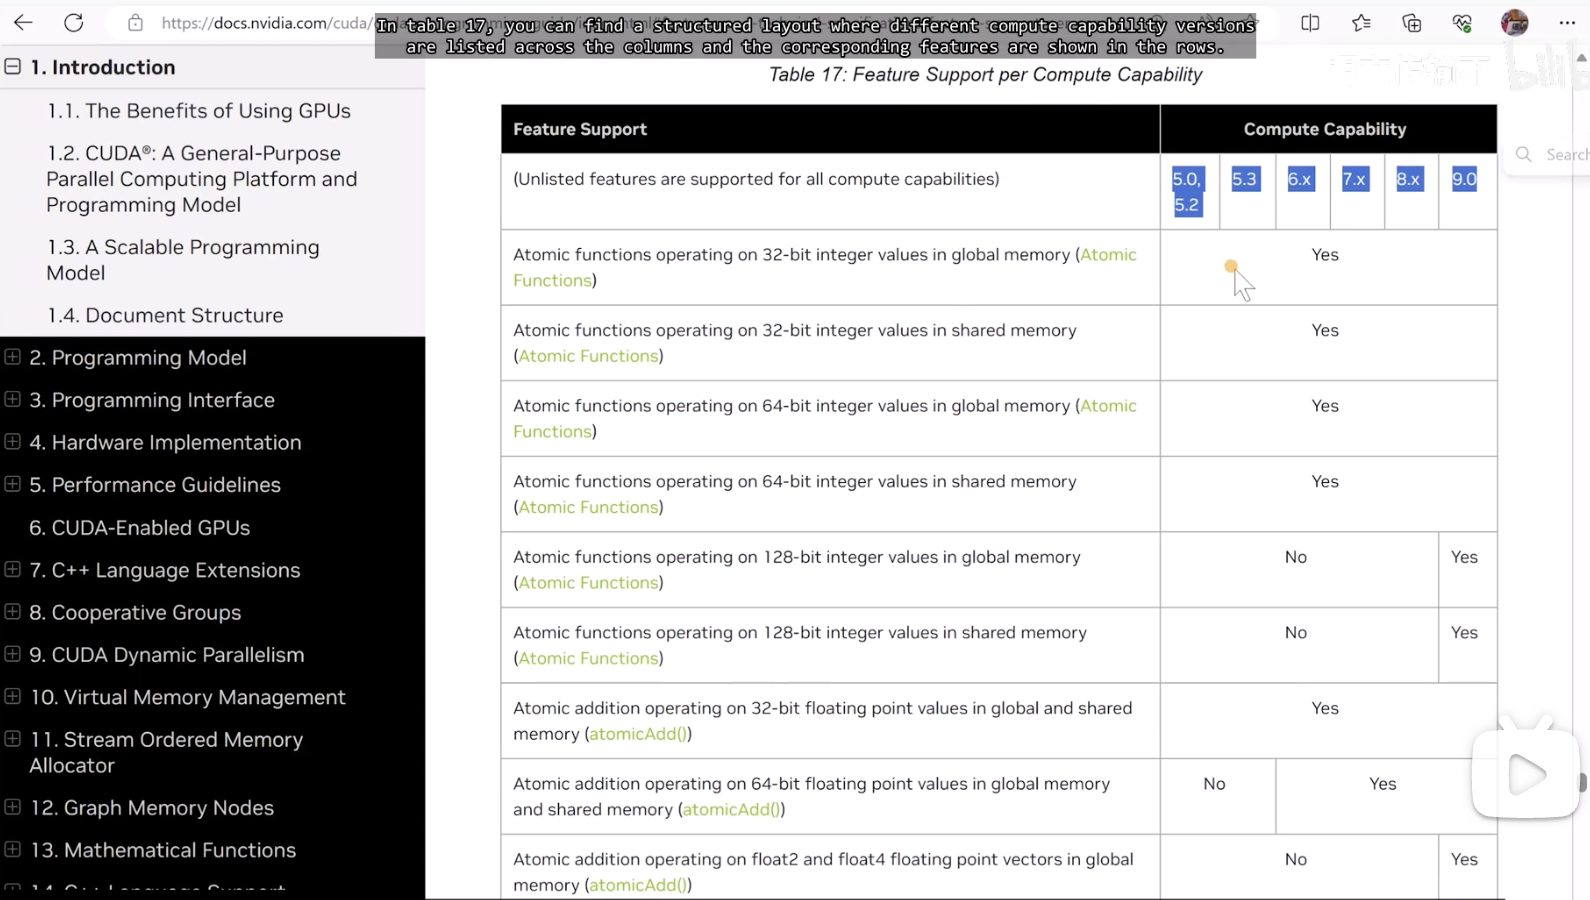
\includegraphics[width=0.75\linewidth]{resources/cuda-041.png}
    \caption{cuda 编程手册}
    \label{fig:placeholder}
\end{figure}


\begin{figure}
    \centering
    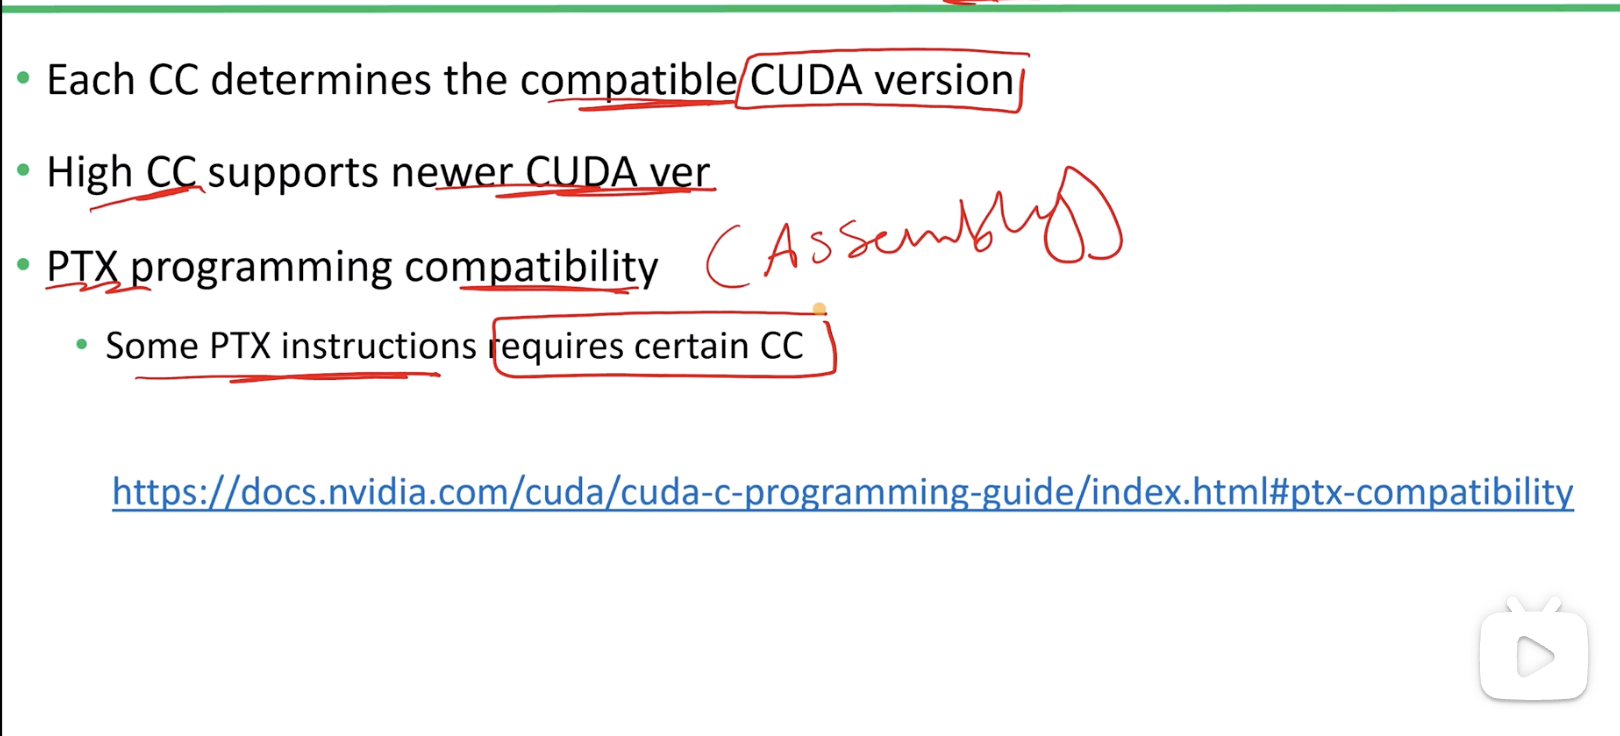
\includegraphics[width=0.75\linewidth]{resources/cuda-042.png}
    \caption{cuda 编程手册}
    \label{fig:placeholder}
\end{figure}


通过链接进入 \href{https://docs.nvidia.com/cuda/cuda-programming-guide/index.html}{CUDA C 编程指南}，你会发现
文档明确指出了某些 PTX 指令对计算能力的版本要求，这些操作或函数仅在计算能力高于 5 的设备上可用。例如 Warp Shuffle 函数
，它能在 Warp 内的线程之间共享数据，而无需使用共享内存或全局内存。

\begin{figure}
    \centering
    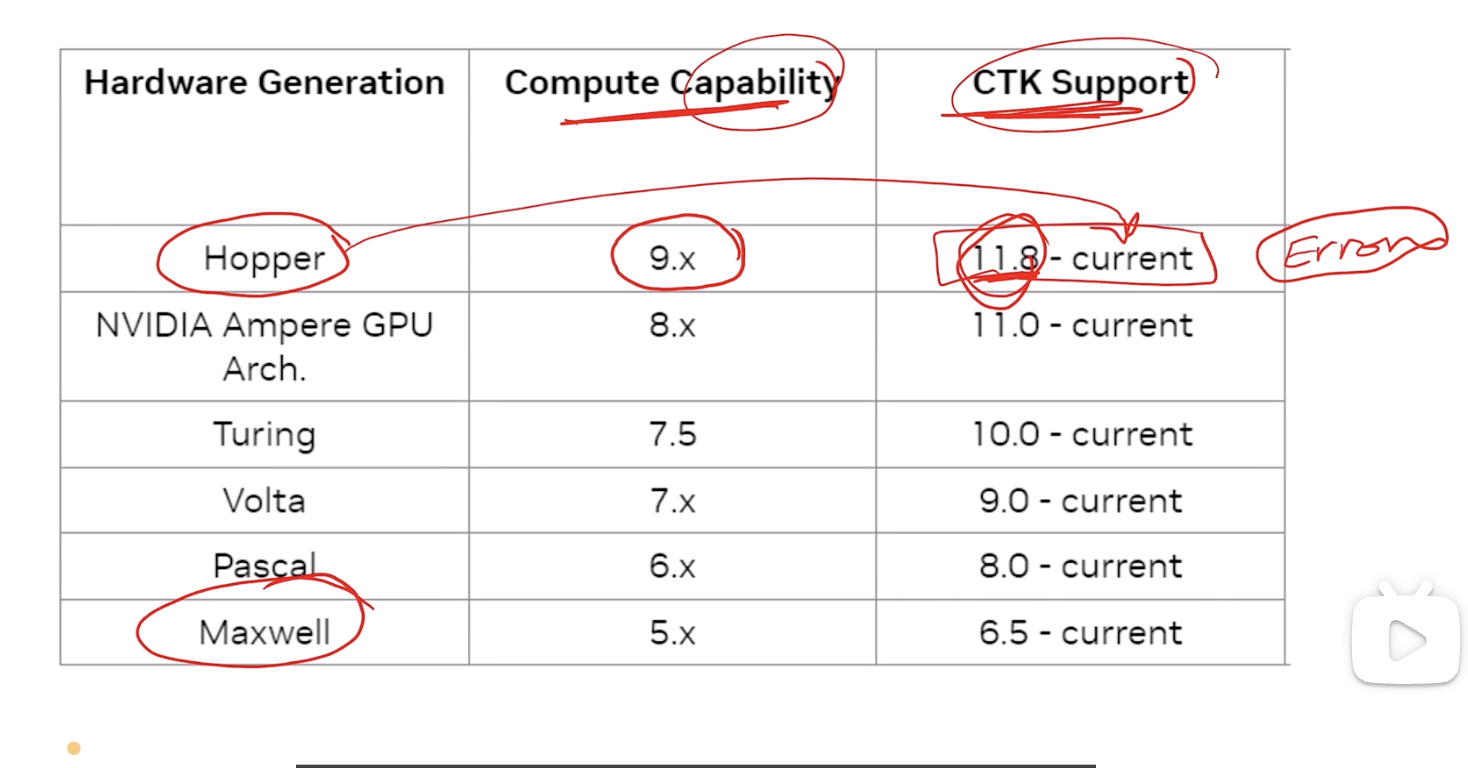
\includegraphics[width=0.75\linewidth]{resources/cuda-043.png}
    \caption{cuda 版本}
    \label{fig:placeholder}
\end{figure}

如果还不够清楚，我们再来看另一个例子。假设你正在从事一个需要最新机器学习技术的项目，你的 GPU 的计算能力将决定你能否使用
最新的 CUDA 工具包——该工具包包含最新的功能和性能优化，可能正是你的应用所需的。

再比如说，如果你使用的是 Hopper 架构的 GPU（目前全球最新一代 GPU 之一），那么对应的计算能力为 9.x。如本表所示，这不仅仅是
对前几代产品的小幅升级，意味着 Hopper GPU 已准备好处理最先进的计算任务。它对 CUDA 工具包的最低版本要求为 11.8，因此在
Hopper 架构中无法使用低于 11.8 的 CUDA 版本。类似地，Maxwell 架构的计算能力编号为 5.x，其最低 CUDA 工具包版本要求为
6.5——如果版本不兼容，你会收到错误提示。

如本表所示，计算能力与所支持的 CUDA 版本之间的关系是理解如何使硬件选择与软件需求相匹配的关键。无论你是开发者、研究人
员，还是依赖 GPU 进行高强度任务的用户，了解这一关系都有助于确保项目运行顺畅、高效并避免意外问题。最后，你可以在此处展
示的网页上发现专为不同应用场景设计的各类 GPU，每一款 GPU 都附带其对应的计算能力，详情见各表格。
